Nesse capítulo serão realizados os laboratórios 7, 8, 9 e 10. Mais algumas
aplicações em biologia são desenvolvidas.

\begin{enumerate}[label=\textbf{Lab \arabic*:}]
    \setcounter{enumi}{6}

    \item Modelo para Epidemia 
    
    Nesse laboratório, um simples modelo compartimental SEIR é desenvolvido
    segundo a figura \ref{fig1:seir}. Um controle da epidemia através da
    vacinação é considerado. É uma simplificação que permite tirar conclusões
    similares àquelas obtidas pela comunidade científica. 

    \begin{figure}[hb]
        \center
        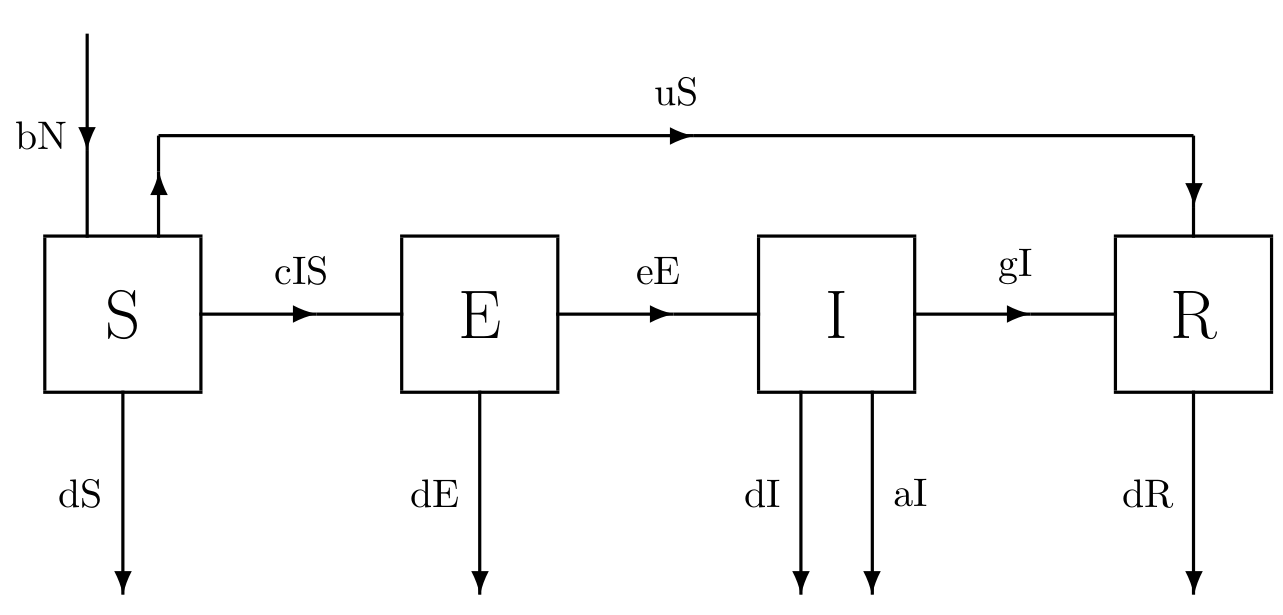
\includegraphics[width = \textwidth]{../images/flow-chat-seir.png}
        \caption{O gráfico de fluxo do modelo é explicado aqui.}
        \label{fig1:seir}
    \end{figure}

    \item Tratamento HIV
    
    Nesse laboratório é estudado a estratégia de tratamento por quimioterapia
    de inibidores da transcrição reversa para o HIV, considerando o sistema
    imunológico do indivíduo, em especial as células CD4+ T que são as mais
    afetadas no processo. A ideia desse controle é inibir a infecciosidade dos
    vírus livres em infectar células suscetíveis. 
    
    \item População de Ursos

    A população de ursos em um parque genérico com proximidade a áreas
    habitadas por humanos é considerada, de forma que essas regiões são
    compartilhadas, o que permite encontros indesejados entre ursos e humanos.
    A caça de ursos tanto na floresta quanto no parque são levados em
    consideração como forma de controle. 

    \item Modelo de Glucose 
    
    Alguns sistemas de equações diferenciais são sensíveis a mudanças nos
    parâmetros. Isso pode até levar a falta de convergência, dentre outros
    problemas. Neste laboratório, examinamos um problema mal condicionado. O
    modelo considerado tem o objetivo de melhorar a habilidade do teste GTT
    para detectar pré-diabetes e diabetes menos severas. especial considera a
    concentração de glucose no sangue e a concentração hormonal líquida. 
 
\end{enumerate}